\documentclass{article}
%packages
% \usepackage{tocloft}
\usepackage{polski}
\usepackage{amsmath}
\usepackage[utf8]{inputenc}
\usepackage{graphicx}
\usepackage{indentfirst}
\usepackage{float}
\usepackage[font=small,labelfont=bf]{caption}
\usepackage[polish]{babel}
\usepackage{hyperref}
\hypersetup{
    colorlinks,
    citecolor=black,
    filecolor=black,
    linkcolor=black,
    urlcolor=black
}
% Variables
\newcommand{\HRule}{\rule{\linewidth}{0.5mm}}
\newcommand{\Prowadzacy}{dr hab. inż. Robert \textsc{Nowicki} prof. PCz}
\newcommand{\Ja}{Piotr \textsc{Filek}\\101311\\I grupa}
\newcommand{\DataLaboratorium}{15 października 2013}
\newcommand{\Uczelnia}{ \textsc{\LARGE Politechnika Częstochowska}\\[1.5cm]}
\newcommand{\Przedmiot}{ \textsc{\Large Podstawy Sieci Komputerowych}\\[1.5cm]}
\newcommand{\TytulLaboratirum}{Laboratorium 2\\Sieci współdzielone}
\frenchspacing


\begin{document}
\begin{titlepage}
\begin{center}
\Uczelnia
% \textsc{\LARGE Politechnika Częstochowska}\\[1.5cm]
\Przedmiot% \textsc{\Large Final year project}\\[0.5cm]
\HRule\\[0.4cm]
{ \huge \bfseries \TytulLaboratirum \\[0.4cm] }
% { \huge \bfseries Large brewing techniques \\[0.4cm]}
\HRule\\[1.5cm]

% Author and supervisor
\begin{minipage}[t]{0.4\textwidth}
\begin{flushleft}\large
\emph{Autor:}\\
\Ja
\end{flushleft}
\end{minipage}
\begin{minipage}[t]{0.5\textwidth}
\begin{flushright} \large
\emph{Prowadzący:} \\
\Prowadzacy
\end{flushright}
\end{minipage}

\vfill

% Bottom of the page
{\large \DataLaboratorium}

\end{center}
\end{titlepage}
\newpage
\section{Cel laboratorium}
Celem laboratorium było zapoznanie się z działaniem sieci przełączanej w porównaniu z siecią współdzieloną technologii Ethernet. Cel ten został uzyskany poprzez porównanie następujących przypadków:
\begin{itemize}
\item sieć współdzielona o architekturze równorzędnej (ang. \textit{peer to peer}),
\item sieć współdzielona o architekturze klient-serwer,
\item siec przełączana o architekturze równorzędnej (ang. \textit{peer to peer}),
\item sieć przełączana o architekturze klient-serwer.
\end{itemize}
Zbadany został także wpływ liczby stacji oraz natężenia ruchu w sieci.
\section{Wyniki}
\begin{figure}[H]
  \centering
  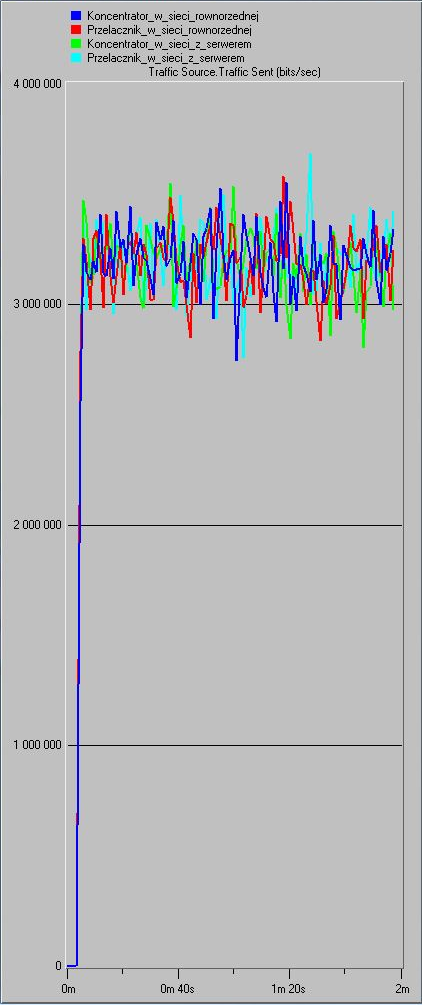
\includegraphics[width=0.58\textwidth]{screens/2_sent.png}
 \caption{Wykres przedstawiający ilość bitów/sec wysłanych dla sieci z 2 stacjami roboczymi.}
 \label{fig:2stacjes}
\end{figure}

\begin{figure}[H]
  \centering
  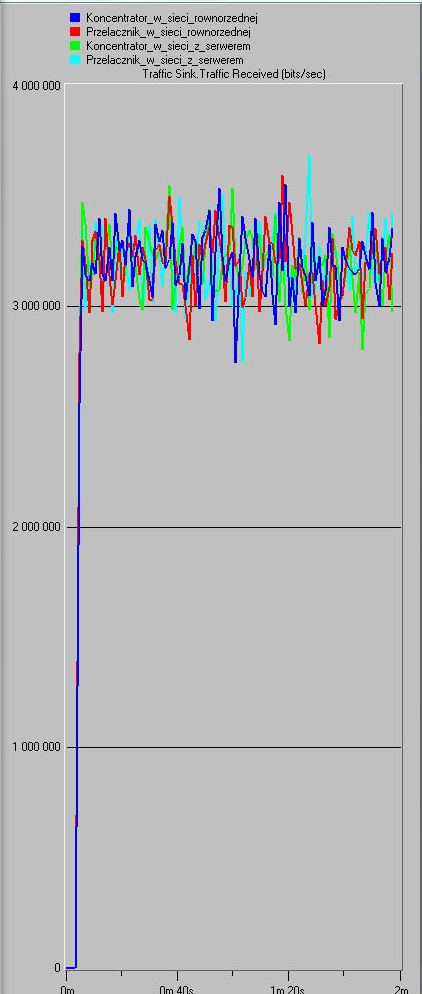
\includegraphics[width=0.60\textwidth]{screens/2_recv.png}
 \caption{Wykres przedstawiający ilość bitów/sec odebranych dla sieci z 2 stacjami roboczymi.}
 \label{fig:2stacjer}
\end{figure}

\begin{figure}[H]
  \centering
  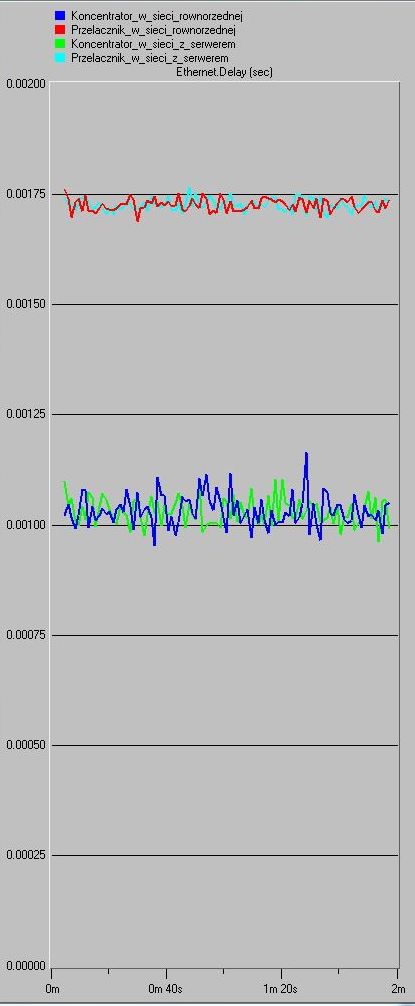
\includegraphics[width=0.60\textwidth]{screens/2_delay.png}
 \caption{Wykres przedstawiający opóźnienia dla sieci z 2 stacjami roboczymi.}
 \label{fig:2stacjed}
\end{figure}


\begin{figure}[H]
  \centering
  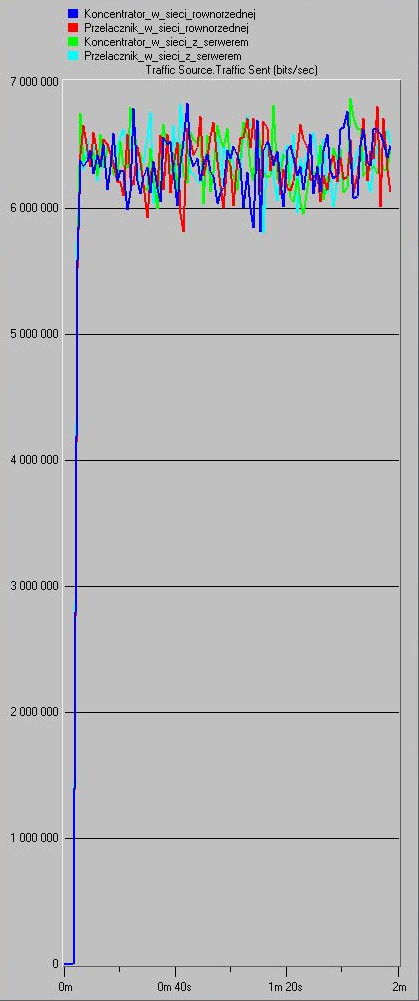
\includegraphics[width=0.60\textwidth]{screens/4_sent.png}
 \caption{Wykres przedstawiający ilość bitów/sec wysłanych dla sieci z 4 stacjami roboczymi.}
 \label{fig:4stacjes}
\end{figure}

\begin{figure}[H]
  \centering
  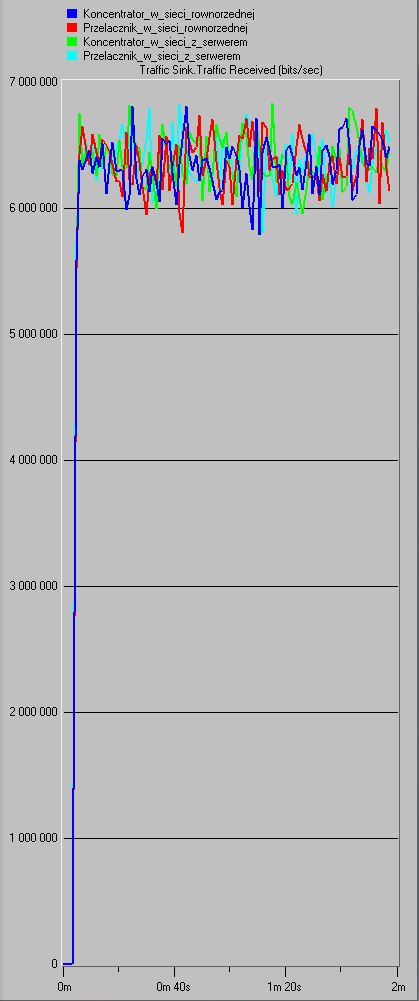
\includegraphics[width=0.60\textwidth]{screens/4_recv.png}
 \caption{Wykres przedstawiający ilość bitów/sec odebranych dla sieci z 4 stacjami roboczymi.}
 \label{fig:4stacjer}
\end{figure}

\begin{figure}[H]
  \centering
  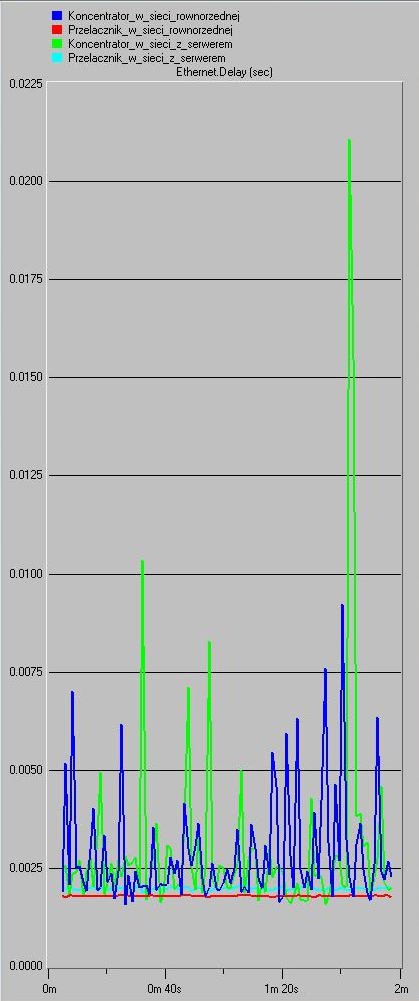
\includegraphics[width=0.60\textwidth]{screens/4_delay.png}
 \caption{Wykres przedstawiający opóźnienia dla sieci z 4 stacjami roboczymi.}
 \label{fig:4stacjed}
\end{figure}


\begin{figure}[H]
  \centering
  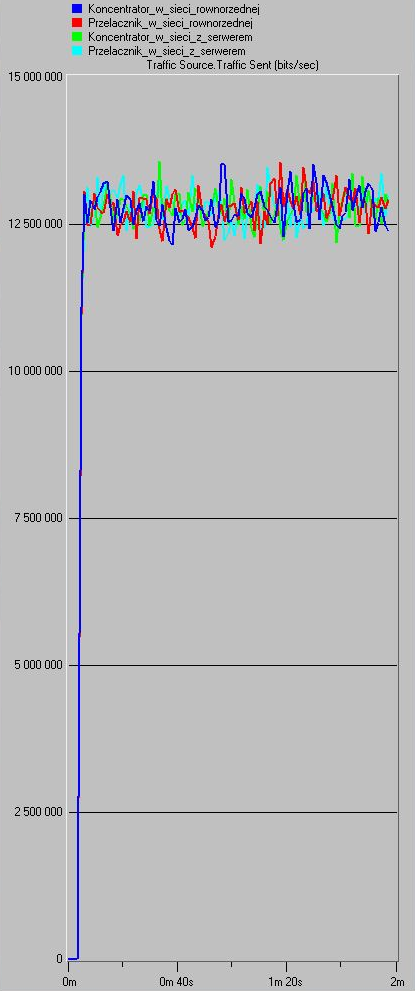
\includegraphics[width=0.60\textwidth]{screens/8_sent.png}
 \caption{Wykres przedstawiający ilość bitów/sec wysłanych dla sieci z 8 stacjami roboczymi.}
 \label{fig:2stacjes}
\end{figure}

\begin{figure}[H]
  \centering
  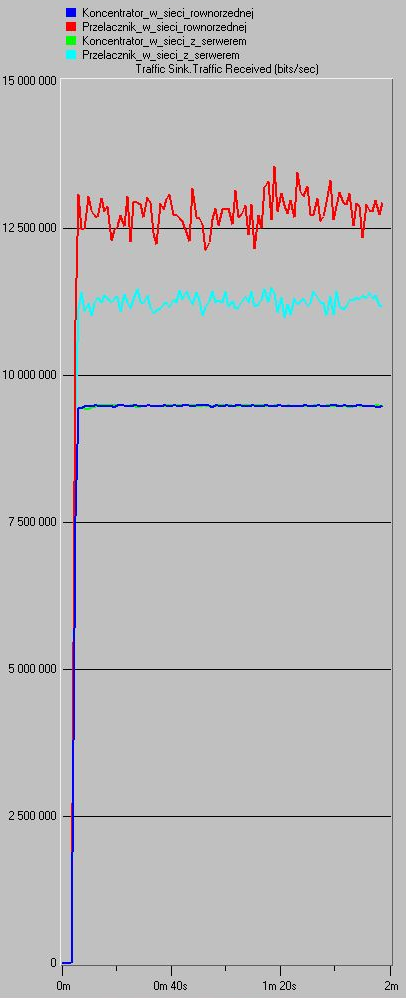
\includegraphics[width=0.60\textwidth]{screens/8_recv.png}
 \caption{Wykres przedstawiający ilość bitów/sec odebranych dla sieci z 8 stacjami roboczymi.}
 \label{fig:8stacjer}
\end{figure}

\begin{figure}[H]
  \centering
  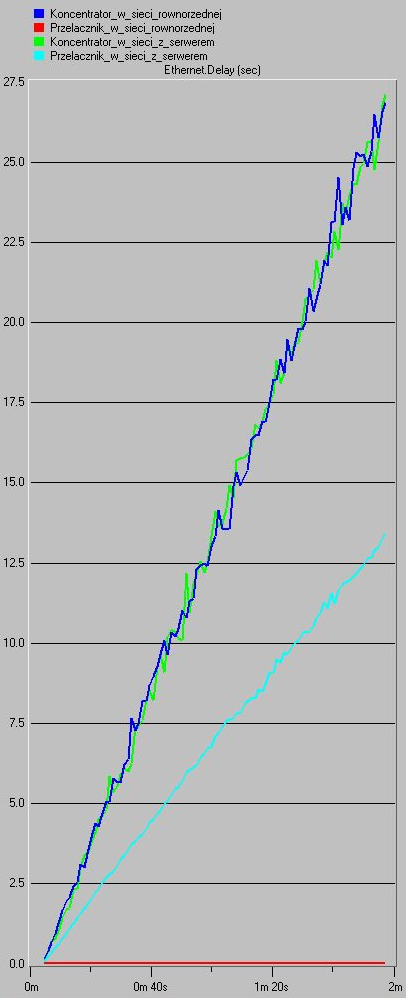
\includegraphics[width=0.60\textwidth]{screens/8_delay.png}
 \caption{Wykres przedstawiający opóźnienia dla sieci z 8 stacjami roboczymi.}
 \label{fig:8stacjed}
\end{figure}


\begin{figure}[H]
  \centering
  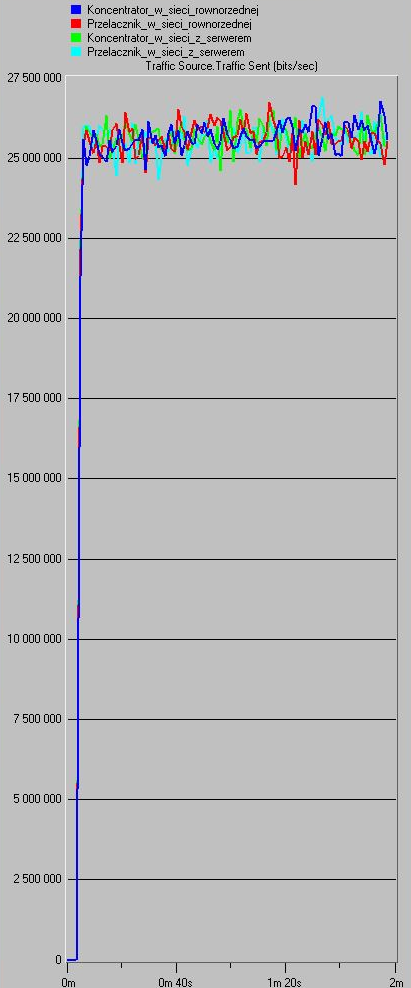
\includegraphics[width=0.60\textwidth]{screens/16_sent.png}
 \caption{Wykres przedstawiający ilość bitów/sec wysłanych dla sieci z 16 stacjami roboczymi.}
 \label{fig:2stacjes}
\end{figure}

\begin{figure}[H]
  \centering
  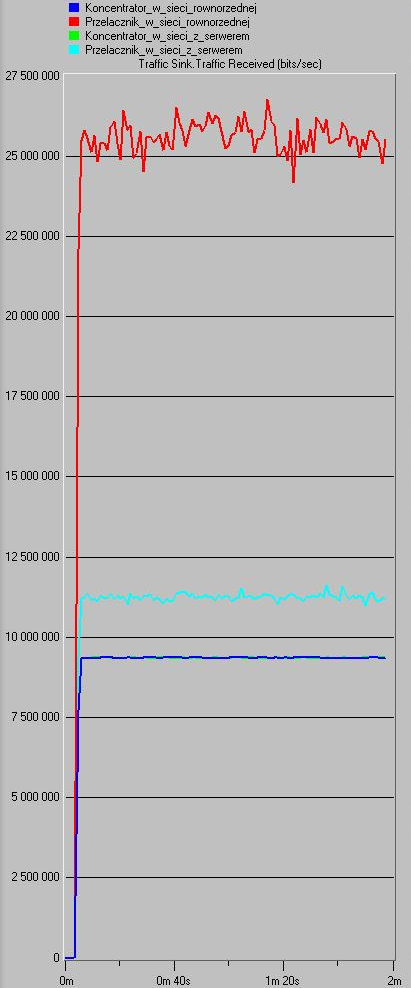
\includegraphics[width=0.60\textwidth]{screens/16_recv.png}
 \caption{Wykres przedstawiający ilość bitów/sec odebranych dla sieci z 16 stacjami roboczymi.}
 \label{fig:16stacjer}
\end{figure}

\begin{figure}[H]
  \centering
  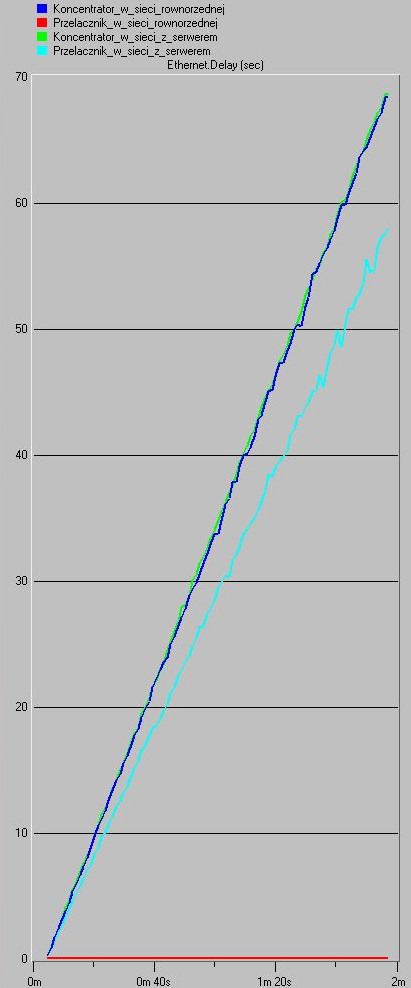
\includegraphics[width=0.60\textwidth]{screens/16_delay.png}
 \caption{Wykres przedstawiający opóźnienia dla sieci z 16 stacjami roboczymi.}
 \label{fig:16stacjed}
\end{figure}



\begin{figure}[H]
  \centering
  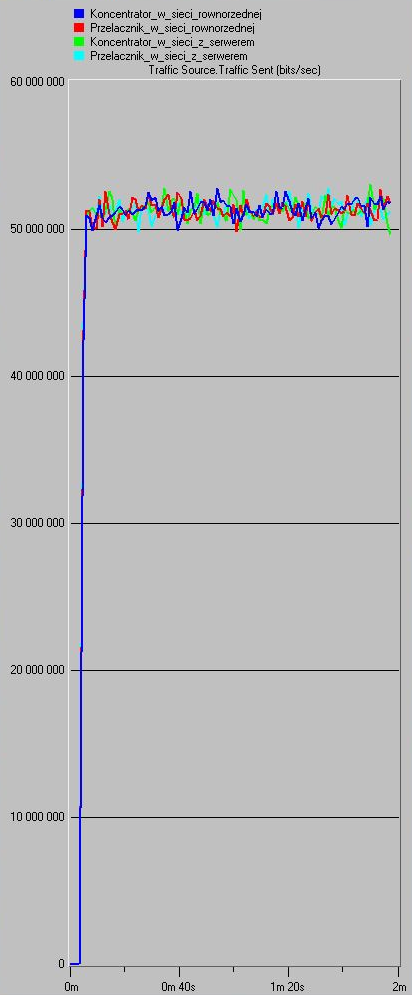
\includegraphics[width=0.60\textwidth]{screens/32_sent.png}
 \caption{Wykres przedstawiający ilość bitów/sec wysłanych dla sieci z 32 stacjami roboczymi.}
 \label{fig:2stacjes}
\end{figure}

\begin{figure}[H]
  \centering
  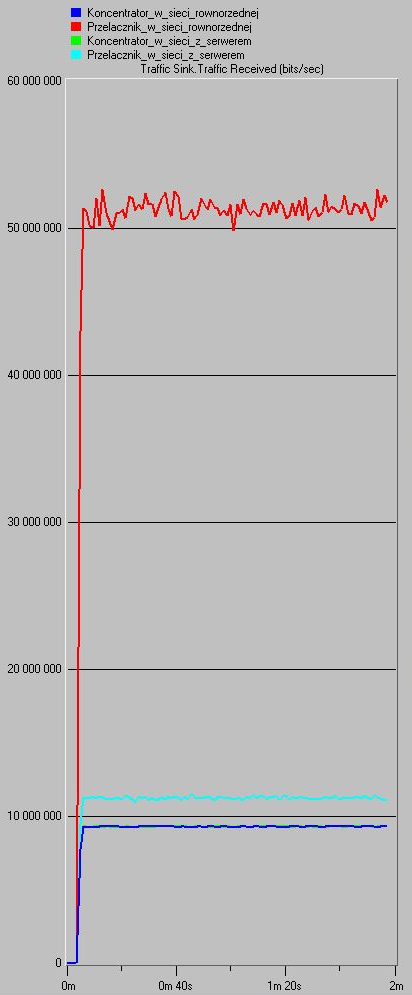
\includegraphics[width=0.60\textwidth]{screens/32_recv.png}
 \caption{Wykres przedstawiający ilość bitów/sec odebranych dla sieci z 32 stacjami roboczymi.}
 \label{fig:32stacjer}
\end{figure}

\begin{figure}[H]
  \centering
  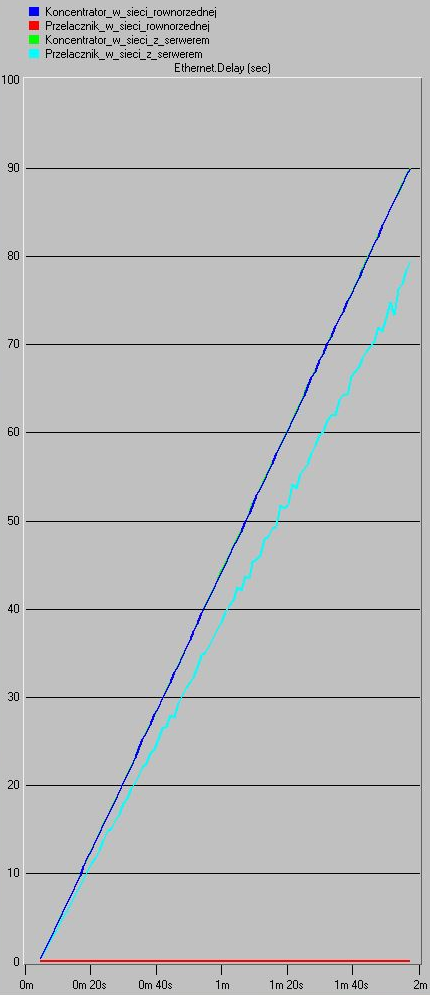
\includegraphics[width=0.60\textwidth]{screens/32_delay.png}
 \caption{Wykres przedstawiający opóźnienia dla sieci z 32 stacjami roboczymi.}
 \label{fig:32stacjed}
\end{figure}




% \begin{figure}[H]
%   \centering
%   \includegraphics[width=0.60\textwidth]{screens/4Stacje.JPG}
%  \caption{Wykresy przedstawiające ruch w sieci oraz opóźnienia dla 4 stacji roboczych. }
%  \label{fig:2stacje}
% \end{figure}

% \begin{figure}[H]
%   \centering
%   \includegraphics[width=0.60\textwidth]{screens/8Stacji.JPG}
%  \caption{Wykresy przedstawiające ruch w sieci oraz opóźnienia dla 8 stacji roboczych. }
%  \label{fig:2stacje}
% \end{figure}

% \begin{figure}[H]
%   \centering
%   \includegraphics[width=0.60\textwidth]{screens/16Stacje.JPG}
%  \caption{Wykresy przedstawiające ruch w sieci oraz opóźnienia dla 16 stacji roboczych. }
%  \label{fig:2stacje}
% \end{figure}

% \begin{figure}[H]
%   \centering
%   \includegraphics[width=1.0\textwidth]{screens/32Stacje.JPG}
%  \caption{Wykresy przedstawiające ruch w sieci oraz opóźnienia dla 32 stacji roboczych. }
%  \label{fig:2stacje}
% \end{figure}


\section{Wnioski}
Przełącznik, (ang. \textit{switch}) w przeciwieństwie do koncentratora (ang. \textit{hub}), nie kopiuje informacji z portu bit-po-bicie, lecz przesyła \emph{ramki} - jest to możliwe dzięki działaniu na drugiej warswie (łącza danych) \emph{modelu OSI}, dzięki czemu jest w stanie przechowywać \emph{adresy MAC} wszystkich urządzeń do niego podłączonych, oraz odpowiednio adresować przesyłane dane - zamiast wysyłać je na wszystkie porty, jak to robi koncentrator. Powoduje to zmniejszenie opóźnień w sieci - jest to szczególnie widoczne w sieci równorzędnej, gdzie opóźnienia są na poziomie zerowym.


\end{document}